\documentclass[a4paper,12pt]{article}
\usepackage[top=3cm, bottom=3cm, left=3cm, right=3cm]{geometry}	%dimension de la feuille
\usepackage[utf8]{inputenc}%codage linux
\usepackage[T1]{fontenc}%les fontes
\usepackage[french]{babel}%caractères français
\usepackage{amsmath}
\usepackage{amssymb}
\usepackage{mathrsfs}
\usepackage{hyperref}%liens pdf
\usepackage{listings}%pour mettre du code
\usepackage{color}%pour la couleur dans le code
\usepackage{graphicx}%pour \includegraphics
\usepackage{float}
\usepackage{longtable}
\usepackage[table]{xcolor}
\lstset{breaklines=true}
\usepackage{verbatim}
\usepackage{array}
\usepackage{svg}

%%%%%%%%%%%%%%%%%%%% Presentation %%%%%%%%%%%%%%%%%%%
\title{Informatique Répartie\\Dossier de Conception\\Sujet : Messagerie instantanée 2}
\author{Ingrid FIQUET\\Morgane LEGROS\\Florian MARTIN\\Thibault THÉOLOGIEN\\Youssef ZERHOUNI ABDOU}
\date{\today}


\begin{document}
\begin{titlepage}
\vfill
	\begin{figure}
	
\includegraphics[scale=0.3]{insarouen-logo.png}
	\end{figure}

\maketitle

\vfill
\noindent \hrulefill

\end{titlepage}


%%%%%%%%%%%%%%%%%%%% Corps %%%%%%%%%%%%%%%%%%%

\newpage
\tableofcontents
\newpage

\section*{Introduction}

L’objectif du projet est de réaliser une application de messagerie instantanée. Il s’agira d’une messagerie permettant à la fois le dialogue vers un utilisateur unique ou bien vers un ensemble d’utilisateurs. La discussion pourra être en audio conférence dans le cas d’un dialogue vers un unique utilisateur. Chaque utilisateur pourra dans les paramètres de son compte gérer la configuration du système de filtrage de la messagerie. 

En ce qui concerne les utilisateurs, la messagerie sera accessible par des utilisateurs humains ou bien par des utilisateurs virtuels. Les utilisateurs virtuels seront capables d’une discussion simple lors d’un dialogue avec un unique utilisateur. Enfin l’administrateur aura lui accès à l’ensemble des comptes utilisateurs et sera le seul autorisé à faire certaines actions telles que bannir un utilisateur par exemple. 

Cette messagerie instantanée sera supportée par tous les OS, accessible via tous les navigateurs et depuis tous types d’appareils (PC, smartphone).


\newpage

\section{Conception préliminaire}

\subsection{Diagramme de modèle du domaine}

\begin{figure}[H]
	\centerline{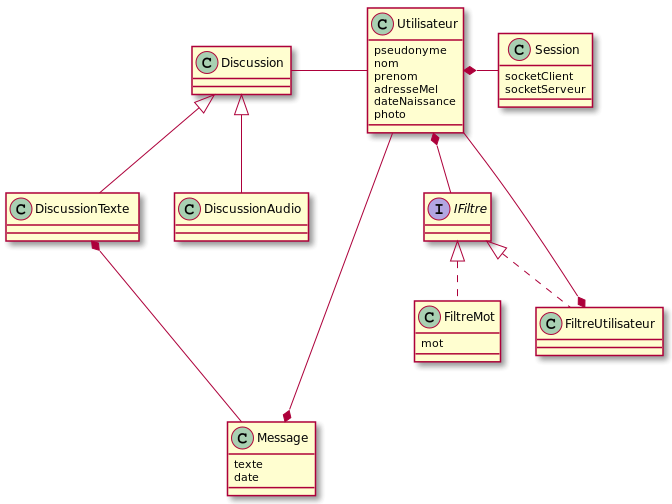
\includegraphics[width=16.5cm]{diagMDC.png}}
	\caption{Diagramme de modèle du domaine côté client}
\end{figure}

\begin{figure}[H]
	\centerline{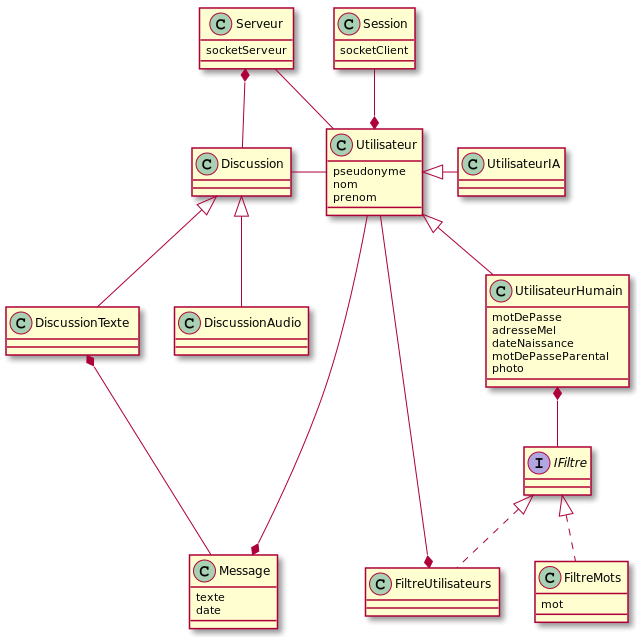
\includegraphics[width=16.5cm]{diagMDS.png}}
	\caption{Diagramme de modèle du domaine côté serveur}
\end{figure}



\subsection{Diagramme de séquence système}

\subsection{Diagramme d'activités de navigation}

\begin{figure}[H]
	\centerline{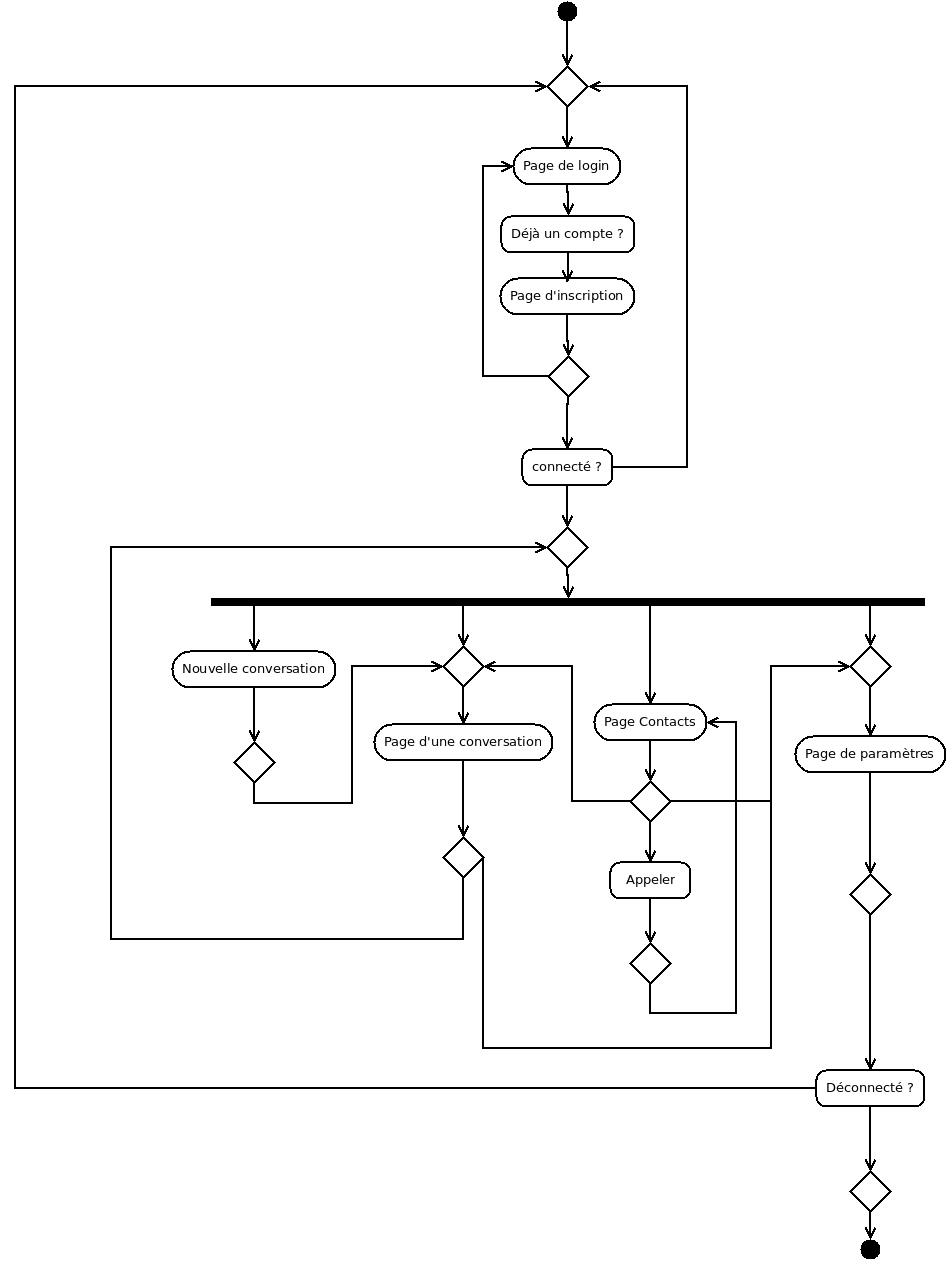
\includegraphics[width=16.5cm]{diagramme_navigationVERSION2.png}}
	\caption{Diagramme de navigation}
\end{figure}

\subsection{Tableau d’Interaction}

\textbf{Tableau d’interaction pour envoyer un message :} \\

Action de début : Vouloir envoyer un message à une personne. \\

\begin{tabular}{|p{7cm}|p{7cm}|}
\hline 
Action de l'utilisateur & Action du système\tabularnewline
\hline 
\hline 
1) Entrer son login et mot de passe (A)  & \tabularnewline
\hline 
2) Valider  & 3) Vérifier le login et le mot de passe dans la base de données\tabularnewline
\hline 
4) Sélectionner une discussion commencée ou cliquer sur le "+" pour
démarrer une conversation avec une nouvelle personne ou aller dans les contacts et cliquer sur l’Icône message en face de la personne correspondante & \tabularnewline
\hline 
5) Envoyer son message  & \tabularnewline
\hline 
\end{tabular}

~\\

Action de fin  : Message affiché dans la discussion. \\

Exception A : Si l'utilisateur n'a pas encore de compte, la première action est de cliquer sur pas encore inscrit, ce qui envoie l'utilisateur sur la page d'inscription où il remplie le formulaire et valide. 



\subsection{Diagramme des classes de conception préliminaire}

\subsection{Un découpage en packages et les signatures externes de chaque package}

\section{Conception détaillée}

%% Détailler par package les élements les constituant. 
%% TODO :
%% - Préciser les attributs et méthodes de classe de toutes les classes participantes et de les regrouper dans un diagramme de classes. 

%% Les méthodes d’un package qui seront considérée comme non triviales devront être commentées et voir leur fonctionnement détaillé par du pseudo-code.

\begin{figure}[H]
	\centerline{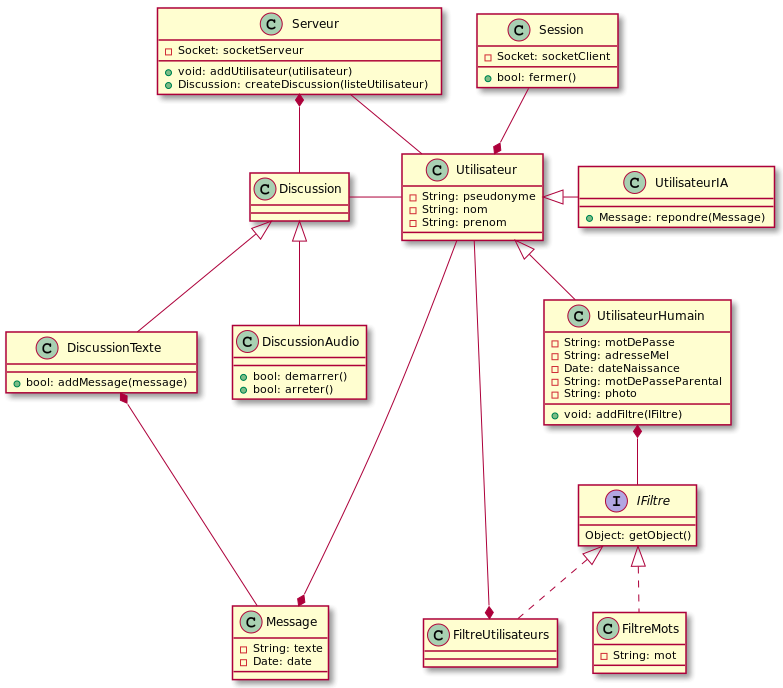
\includegraphics[width=16.5cm]{diagClassServeur.png}}
	\caption{Diagramme de classes}
\end{figure}


\end{document}
